\documentclass[journal,12pt,twocolumn]{IEEEtran}

\usepackage{setspace}
\usepackage{gensymb}

\singlespacing


\usepackage[cmex10]{amsmath}

\usepackage{amsthm}

\usepackage{mathrsfs}
\usepackage{txfonts}
\usepackage{stfloats}
\usepackage{bm}
\usepackage{cite}
\usepackage{cases}
\usepackage{subfig}

\usepackage{longtable}
\usepackage{multirow}

\usepackage{enumitem}
\usepackage{mathtools}
\usepackage{steinmetz}
\usepackage{tikz}
\usepackage{circuitikz}
\usepackage{verbatim}
\usepackage{tfrupee}
\usepackage[breaklinks=true]{hyperref}
\usepackage{graphicx}
\usepackage{tkz-euclide}
\usepackage{float}

\usetikzlibrary{calc,math}
\usepackage{listings}
    \usepackage{color}                                            %%
    \usepackage{array}                                            %%
    \usepackage{longtable}                                        %%
    \usepackage{calc}                                             %%
    \usepackage{multirow}                                         %%
    \usepackage{hhline}                                           %%
    \usepackage{ifthen}                                           %%
    \usepackage{lscape}     
\usepackage{multicol}
\usepackage{chngcntr}

\DeclareMathOperator*{\Res}{Res}

\renewcommand\thesection{\arabic{section}}
\renewcommand\thesubsection{\thesection.\arabic{subsection}}
\renewcommand\thesubsubsection{\thesubsection.\arabic{subsubsection}}

\renewcommand\thesectiondis{\arabic{section}}
\renewcommand\thesubsectiondis{\thesectiondis.\arabic{subsection}}
\renewcommand\thesubsubsectiondis{\thesubsectiondis.\arabic{subsubsection}}


\hyphenation{op-tical net-works semi-conduc-tor}
\def\inputGnumericTable{}                                 %%

\lstset{
%language=C,
frame=single, 
breaklines=true,
columns=fullflexible
}
\begin{document}
\newtheorem{theorem}{Theorem}[section]
\newtheorem{problem}{Problem}
\newtheorem{proposition}{Proposition}[section]
\newtheorem{lemma}{Lemma}[section]
\newtheorem{corollary}[theorem]{Corollary}
\newtheorem{example}{Example}[section]
\newtheorem{definition}[problem]{Definition}

\newcommand{\BEQA}{\begin{eqnarray}}
\newcommand{\EEQA}{\end{eqnarray}}
\newcommand{\define}{\stackrel{\triangle}{=}}
\bibliographystyle{IEEEtran}
\providecommand{\mbf}{\mathbf}
\providecommand{\pr}[1]{\ensuremath{\Pr\left(#1\right)}}
\providecommand{\qfunc}[1]{\ensuremath{Q\left(#1\right)}}
\providecommand{\sbrak}[1]{\ensuremath{{}\left[#1\right]}}
\providecommand{\lsbrak}[1]{\ensuremath{{}\left[#1\right.}}
\providecommand{\rsbrak}[1]{\ensuremath{{}\left.#1\right]}}
\providecommand{\brak}[1]{\ensuremath{\left(#1\right)}}
\providecommand{\lbrak}[1]{\ensuremath{\left(#1\right.}}
\providecommand{\rbrak}[1]{\ensuremath{\left.#1\right)}}
\providecommand{\cbrak}[1]{\ensuremath{\left\{#1\right\}}}
\providecommand{\lcbrak}[1]{\ensuremath{\left\{#1\right.}}
\providecommand{\rcbrak}[1]{\ensuremath{\left.#1\right\}}}
\theoremstyle{remark}
\newtheorem{rem}{Remark}
\newcommand{\sgn}{\mathop{\mathrm{sgn}}}
\providecommand{\abs}[1]{\vert#1\vert}
\providecommand{\res}[1]{\Res\displaylimits_{#1}} 
\providecommand{\norm}[1]{\lVert#1\rVert}
%\providecommand{\norm}[1]{\lVert#1\rVert}
\providecommand{\mtx}[1]{\mathbf{#1}}
\providecommand{\mean}[1]{E[ #1 ]}
\providecommand{\fourier}{\overset{\mathcal{F}}{ \rightleftharpoons}}
%\providecommand{\hilbert}{\overset{\mathcal{H}}{ \rightleftharpoons}}
\providecommand{\system}{\overset{\mathcal{H}}{ \longleftrightarrow}}
	%\newcommand{\solution}[2]{\textbf{Solution:}{#1}}
\newcommand{\solution}{\noindent \textbf{Solution: }}
\newcommand{\cosec}{\,\text{cosec}\,}
\providecommand{\dec}[2]{\ensuremath{\overset{#1}{\underset{#2}{\gtrless}}}}
\newcommand{\myvec}[1]{\ensuremath{\begin{pmatrix}#1\end{pmatrix}}}
\newcommand{\mydet}[1]{\ensuremath{\begin{vmatrix}#1\end{vmatrix}}}
\numberwithin{equation}{subsection}
\makeatletter
\@addtoreset{figure}{problem}
\makeatother
\let\StandardTheFigure\thefigure
\let\vec\mathbf
\renewcommand{\thefigure}{\theproblem}
\def\putbox#1#2#3{\makebox[0in][l]{\makebox[#1][l]{}\raisebox{\baselineskip}[0in][0in]{\raisebox{#2}[0in][0in]{#3}}}}
     \def\rightbox#1{\makebox[0in][r]{#1}}
     \def\centbox#1{\makebox[0in]{#1}}
     \def\topbox#1{\raisebox{-\baselineskip}[0in][0in]{#1}}
     \def\midbox#1{\raisebox{-0.5\baselineskip}[0in][0in]{#1}}
\vspace{3cm}
\title{QUIZ 2}
\author{Ananthoju Pranav Sai \\ AI20BTECH11004}
\maketitle
\newpage
\bigskip
\renewcommand{\thefigure}{\theenumi}
\renewcommand{\thetable}{\theenumi}
Download all python codes from 
\begin{lstlisting}
https://github.com/Ananthoju-Pranav-Sai/EE3900/blob/main/Quiz_2/codes
\end{lstlisting}
%
and latex-tikz codes from 
%
\begin{lstlisting}
https://github.com/Ananthoju-Pranav-Sai/EE3900/tree/main/Quiz_2/Quiz_2.tex
\end{lstlisting}
%
\section{Discrete Time Signal Processing Q 3.21(b)}
Consider an linear time-invariant system with impulse response
\begin{align}
    h[n] = \begin{cases} 
                a^{n} & n\geq 0\\
                0 & n<0
            \end{cases}
\end{align}
and input 
\begin{align}
    x[n] = \begin{cases} 
                1 & 0\leq n\leq (N-1)\\
                0 & otherwise
            \end{cases}
\end{align}
Determine the output $y[n]$ by computing the inverse $z$-transform of the product of the $z$-transforms of $x[n]$ and $h[n]$.
\section{Solution}
Given,
\begin{align}
    h[n] = \begin{cases} 
                a^{n} & n\geq 0\\
                0 & n<0
            \end{cases}
\end{align}
applying $z$-transform
\begin{align}
    H(z) &= \mathcal{Z}(h[n])\\
    \impies H(z) &= \sum_{n=-\infty}^{\infty}h[n]z^{-n}\\
    \implies H(z) &= \sum_{n=0}^{\infty}a^n z^{-n}\\
    \implies H(z) &= \frac{1}{1-az^{-1}}\hspace{1cm}|z|>|a|
\end{align}
input
\begin{align}
    x[n] = \begin{cases} 
                1 & 0\leq n\leq (N-1)\\
                0 & otherwise
            \end{cases}
\end{align}
applying $z$-transform
\begin{align}
    X(z) &= \mathcal{Z}(x[n])\\
    \implies X(z) &= \sum_{n=-\infty}^{\infty}x[n]z^{-n}\\
    \implies X(z) &= \sum_{n=0}^{N-1}z^{-n}\\
    \implies X(z) &= \frac{1-z^{-N}}{1-z^{-1}}
\end{align}
We know 
\begin{align}
    Y(z) &= X(z)H(z)\\
    &= \frac{1-z^{-N}}{(1-z^{-1})(1-az^{-1})}\hspace{1cm} |z|>|a|\\
     &= \frac{1}{(1-z^{-1})(1-az^{-1})}-\frac{z^{-N}}{(1-z^{-1})(1-az^{-1})}    \label{a}
\end{align}
Let, 
\begin{align}
    G(z)&=\frac{1}{(1-az^{-1})(1-z^{-1})}  \label{b} \\
    \implies G(z)&=\brak{\frac{1}{1-a}}\brak{\frac{1}{1-z^{-1}}-\frac{a}{1-az^{-1}}}
\end{align}
applying inverse $z$-transform
\begin{align}
    g[n] &= \mathcal{Z}^{-1}(G(z))\\
    \implies g[n] &= \brak{\frac{1}{1-a}}(u[n]-a(a^nu[n]))\\
    \implies g[n] &= \brak{\frac{1-a^{n+1}}{1-a}}u[n] \label{c}
\end{align}
from $\eqref{a}$ and $\eqref{b}$ we have
\begin{align}
    Y(z) = G(z)-z^{-N}G(z)
\end{align}
applying inverse $z$-transform
\begin{align}
    y[n] &= \mathcal{Z}^{-1}(Y(z))\\
    \implies y[n] &= \mathcal{Z}^{-1}(G(z))-\mathcal{Z}^{-1}(z^{-N}G(z))\\
    \implies y[n] &= g[n]-g[n-N]
\end{align}
from $\eqref{c}$ we have
\begin{align}
    y[n] &= \brak{\frac{1-a^{n+1}}{1-a}}u[n]-\brak{\frac{1-a^{n-N+1}}{1-a}}u[n-N]
\end{align}
\begin{figure}[!ht]
    \centering
    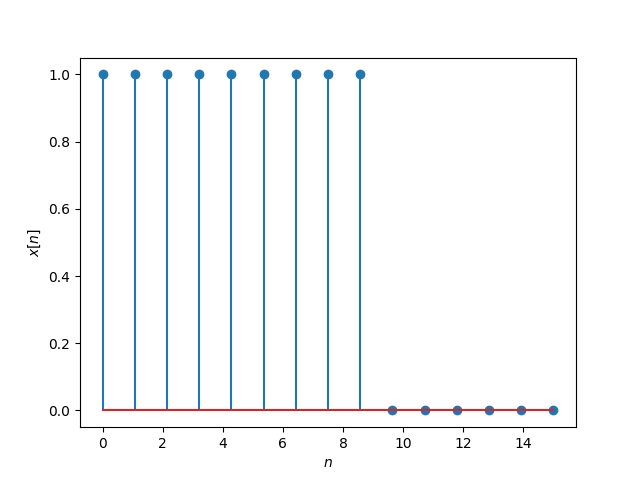
\includegraphics[width=\columnwidth]{x[n]_plot.png}
    \caption{Plot of input signal x[n] for N=10}
    \label{x[n]_plot}
\end{figure}
\begin{figure}[!ht]
    \centering
    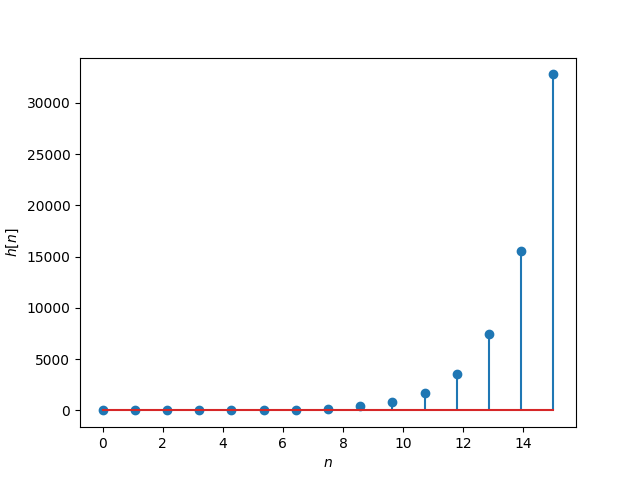
\includegraphics[width=\columnwidth]{h[n]_plot.png}
    \caption{Plot of impulse response h[n] for a=2}
    \label{h[n]_plot}
\end{figure}
\begin{figure}[H]
    \centering
    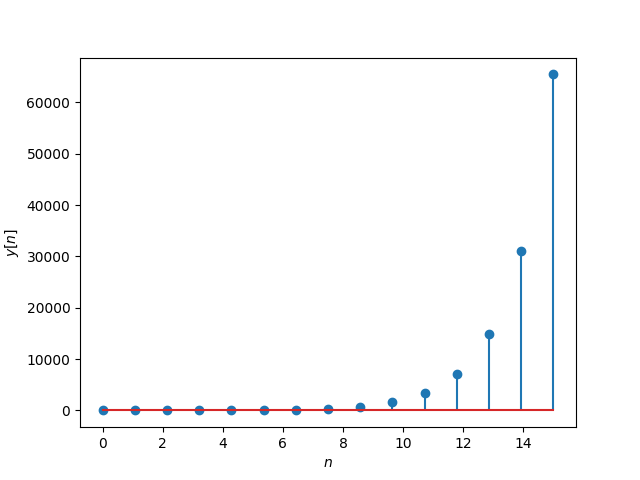
\includegraphics[width=\columnwidth]{y[n]_plot.png}
    \caption{Plot of output signal y[n] for a=2 and N=10}
    \label{y[n]_plot}
\end{figure}
\end{document}